%!TEX root = dissertacao.tex
\section{PROPRIEDADES ESTÁTICAS}
\label{sec:propriedadeEstaticasDef}
Em ACs, propriedades estáticas são propriedades computadas com base nas tabelas de transições. Essas propriedades permitem prever determinados comportamentos de ACs sem consultar sua evolução espaço-temporal. 

Esta seção descreve algumas propriedades estáticas que já têm seus algoritmos geradores de templates implementados na biblioteca \textit{CATemplates} \cite{CATemplates}.

\subsection{Conservabilidade de Estados e Conservabilidade de Paridade}
\label{sec:propriedadeEstaticasDefCon}
Conservabilidade de estados é uma propriedade estática que determina que a soma dos estados de um determinado autômato celular não deve se alterar durante a evolução espaço-temporal, independente da configuração inicial.

De acordo com Boccara e Fukś (\citeyear{boccara2002}), um AC é conservativo quando cada uma de suas regras locais $f$ de vizinhança $(\alpha_0,\alpha_1, \dots, \alpha_{n-1})$ respeita as condições descritas na Eq. \eqref{eq:conservativeCA}.

\begin{equation}
\begin{split}
f(\alpha_0,\alpha_1, \dots,\alpha_{n-1}) = \alpha_0 + (\sum_{i=0}^{n-2}f(0_0,0_1, \dots,0_i,\alpha_1,\alpha_2, \dots,\alpha_{n-1}) \\- f(0_0,0_1, \dots,0_i,\alpha_0,\alpha_1, \dots,\alpha_{n-i-1}))
\label{eq:conservativeCA}
\end{split}
\end{equation}

Para exemplificar, considere-se a regra 204 do espaço elementar. Por meio da condição mostrada na Eq. \eqref{eq:conservativeCA}, será provado que essa regra é conservativa, já que satisfaz a condição. A Eq. \eqref{eq:ruleTable204} representa a tabela de transições da regra 204.

\begin{equation}
\begin{split}
(((1,1,1),1),((1,1,0),1),\\((1,0,1),0),((1,0,0),0),\\((0,1,1),1),((0,1,0),1),\\((0,0,1),0),((0,0,0),0))
\label{eq:ruleTable204}
\end{split}
\end{equation}

Como demonstra \citeonline{Verardo2014}, a aplicação das condições da Eq. \eqref{eq:conservativeCA} nas tabelas de transições de ACs do espaço elementar, resulta no sistema descrito pela Eq. \eqref{eq:conservativeLinearSystem}.

\begin{equation}
\left\{\begin{matrix}
 f(0,0,0) = 0 + (f(0,0,0) - f(0,0,0)) + (f(0,0,0) - f(0,0,0))\\ 
 f(0,0,1) = 0 + (f(0,0,1) - f(0,0,0)) + (f(0,0,0) - f(0,0,0))\\ 
 f(0,1,0) = 0 + (f(0,1,0) - f(0,0,1)) + (f(0,0,1) - f(0,0,0))\\ 
 f(0,1,1) = 0 + (f(0,1,1) - f(0,0,1)) + (f(0,0,1) - f(0,0,0))\\ 
 f(1,0,0) = 1 + (f(0,0,0) - f(0,1,0)) + (f(0,0,0) - f(0,0,1))\\ 
 f(1,0,1) = 1 + (f(0,0,1) - f(0,1,0)) + (f(0,0,0) - f(0,0,1))\\ 
 f(1,1,0) = 1 + (f(0,1,0) - f(0,1,1)) + (f(0,0,1) - f(0,0,1))\\ 
 f(1,1,1) = 1 + (f(0,1,1) - f(0,1,1)) + (f(0,0,1) - f(0,0,1))
\end{matrix}\right.
\label{eq:conservativeLinearSystem}
\end{equation}

A Eq. \eqref{eq:conservativeLinearSystem} simplificada é representada pela Eq. \eqref{eq:conservativeLinearSystem2}.

\begin{equation}
\left\{\begin{matrix}
 f(0,0,0) & = & 0 		& &\\ 
 f(0,0,1) & = & f(0,0,1)& & \\ 
 f(0,1,0) & = & f(0,1,0)& & \\ 
 f(0,1,1) & = & f(0,1,1)& & \\ 
 f(1,0,0) & = & 1 - f(0,0,1) - f(0,1,0) \\ 
 f(1,0,1) & = & 1 - f(0,1,0) \\ 
 f(1,1,0) & = & 1 + (f(0,1,0) - f(0,1,1))\\ 
 f(1,1,1) & = & 1 & &
\end{matrix}\right.
\label{eq:conservativeLinearSystem2}
\end{equation}

Excluindo-se as condições tautológicas do sistema e atribuindo os valores das funções locais $f$ conforme a tabela de transições da regra 204, é obtido o sistema descrito pela Eq. \eqref{eq:conservativeAC204}. Esse sistema, ao não apresentar condições contraditórias ou falsas, prova que a regra 204 é conservativa.

\begin{equation}
\left\{\begin{matrix}
 0 & = & 0 \\ 
 0 & = & 1 - 0 - 1 \\ 
 0 & = & 1 - 1 \\ 
 1 & = & 1 + (1 - 1)\\ 
 1 & = & 1 
\end{matrix}\right.
\label{eq:conservativeAC204}
\end{equation}

O processo de gerar regras conservativas de paridade é bem parecido. Porém, as condições estabelecidas por Boccara e Fukś (\citeyear{boccara2002}) são ligeiramente modificadas em relação à Eq. \eqref{eq:conservativeCA}, de forma que cada uma das funções locais deve respeitar agora as condições da Eq. \eqref{eq:parityConservativeCA}.
\begin{equation}
\begin{split}
f(\alpha_0,\alpha_1, \dots,\alpha_{n-1}) \equiv \alpha_0 + (\sum_{i=0}^{n-2}f(0_0,0_1, \dots,0_i,\alpha_1,\alpha_2, \dots,\alpha_{n-1}) \\- f(0_0,0_1, \dots,0_i,\alpha_0,\alpha_1, \dots,\alpha_{n-i-1})) \; \mod 2
\label{eq:parityConservativeCA}
\end{split}
\end{equation}


\subsection{Simetria Interna}
Para entender a propriedade de simetria interna faz-se necessário compreender o funcionamento das transformações de regras e classes de equivalência dinâmica. As explicações a seguir são válidas para regras binárias pois o algoritmo implementado no \textit{CATemplates} é para regras binárias, apesar de ser possível sua generalização para $k$ estados.

Dada uma tabela de transições de um AC, existem três transformações que podem ser empregadas e que resultam em ACs com comportamentos dinâmicos equivalentes: \textit{reflexão}, \textit{conjugação} e \textit{composição reflexão-conjugação}. A reflexão é a transformação obtida ao refletir os bits das vizinhanças da tabela. A conjugação é obtida ao inverter todos os estados das células da tabela de transições. Já a composição é a transformação obtida ao se efetuar a reflexão e a conjugação, independente da ordem.

Essas transformações podem ser aplicadas tanto à vizinhança, como também a toda a tabela de transições. Para aplicar uma transformação a toda uma tabela, basta aplicá-la a cada uma das vizinhanças da tabela. Uma tabela, transição ou vizinhança é chamada de invariante a uma transformação caso essa transformação, quando aplicada a ela, não promova nenhum efeito. Um exemplo de vizinhança invariante por reflexão é a vizinhança $(1,0,1)$.

Para exemplificar essas transformações e as equivalências dinâmicas considere-se a tabela de transição da regra 60, ilustrada pela Figura \ref{fig:table60}. Ao aplicar a transformação por reflexão na regra 60 obtém-se a regra 102 do espaço elementar, ilustrada pela Figura \ref{fig:table102}.

	\begin{figure}[h!]
	  \centering
	  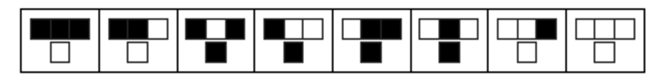
\includegraphics[width=.6\textwidth]{fig_ruleIcon60.pdf}
	  \caption{Tabela de transições da regra 60 do espaço elementar.}
	  \label{fig:table60}
	\end{figure}

	\begin{figure}[h!]
	  \centering
	  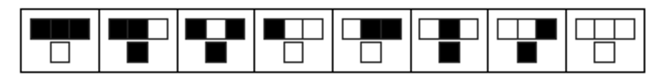
\includegraphics[width=.6\textwidth]{fig_ruleIcon102.pdf}
	  \caption{Tabela de transições da regra 102 do espaço elementar, obtida através da transformação de reflexão aplicada na tabela de transições da regra 60.}
	  \label{fig:table102}
	\end{figure}

Ao aplicar a transformação por conjugação na regra 60 obtém-se a regra 195 do espaço elementar, conforme ilustrado na Figura \ref{fig:table195}. Por fim, ao aplicar a transformação por composição de reflexão e conjugação na regra 60 obtém-se a regra 153 do espaço elementar, conforme ilustrado na Figura \ref{fig:table153}.

	\begin{figure}[h!]
	  \centering
	  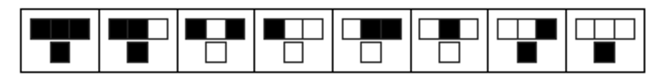
\includegraphics[width=.6\textwidth]{fig_ruleIcon195.pdf}
	  \caption{Tabela de transições da regra 195 do espaço elementar, obtida através da transformação de conjugação aplicada na tabela de transições da regra 60.}
	  \label{fig:table195}
	\end{figure}

	\begin{figure}[h!]
	  \centering
	  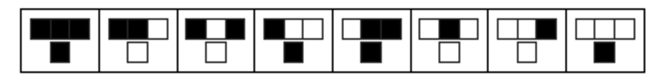
\includegraphics[width=.6\textwidth]{fig_ruleIcon153.pdf}
	  \caption{Tabela de transições da regra 153 do espaço elementar, obtida através da transformação de composição aplicada na tabela de transições da regra 60.}
	  \label{fig:table153}
	\end{figure}

Tanto a regra 60, como as regras 102, 153 e 195 pertencem à mesma classe de equivalência dinâmica. Uma forma interessante de entender o porquê é analisando a evolução espaço-temporal dessas regras, ilustrada pela Figura \ref{fig:dynamicEquivalecy}.

	\begin{figure}[h!]
	  \centering
	  \def\svgscale{0.45}
	  \import{./img/}{fig_ruleEquivalence60.pdf_tex}
	  \caption{Evolução espaço-temporal das regras pertencente à mesma classe dinâmica da regra 60.}
	  \label{fig:dynamicEquivalecy}
	\end{figure}

Tendo em vista as tabelas de transições obtidas por meio das transformações, é possível saber quão simétrica é uma regra em relação a uma determinada transformação ou, em outras palavras, qual o grau de simetria interna de uma regra em relação à transformação em questão. A simetria interna pode ser representada pelo número de vizinhanças que permanecem iguais após aplicada uma determinada transformação. Exemplificando, a regra 60 dos ACs elementares tem valor de simetria interna por reflexão igual a 4, pois compartilha as transições de estado $((1,1,1),0)$, $((1,0,1),1)$, $((0,1,0),1)$ e $ ((0,0,0),0)$ com a regra resultante de sua transformação por reflexão, a regra 102. Vale notar que, como as vizinhanças compartilhadas são todas e apenas as vizinhanças invariantes do espaço elementar, logo pode-se dizer que a regra 60 tem a menor simetria interna possível para o espaço elementar.

Um resultado bem diferente pode ser visto ao se repetir esse mesmo processo para a regra 204, que tem valor 8 de simetria interna para transformação por reflexão. Esse valor é máximo possível para o espaço elementar e evidencia que, ao se aplicar a transformação por reflexão na regra 204, será obtida a mesma regra como resultado. Uma regra que possua máxima simetria para uma transformação é uma regra invariante.

Vale frisar que apenas transformações por reflexão apresentam vizinhanças invariantes. No caso das reflexões por conjugação e por composição isso não ocorre.


\subsection{Totalidade e Semi-totalidade}
\label{sec:propriedadeEstaticasDefTot}
Os ACs totalísticos são autômatos celulares cujo valor de uma célula depende apenas da soma dos valores dos seus vizinhos no passo de tempo anterior \cite{wolfram1983statistical}.

De forma análoga, pode-se considerar que as transições dependem da média dos valores das células que compõem  a vizinhança. A Figura \ref{fig:totalistcRule} ilustra a tabela de transição de um AC totalístico com $k = 3$ e $r = 1$ (especificamente, o de número 777, entre os totalísticos do espaço em questão) \cite{wolfram2002new}.

	\begin{figure}[h!]
	  \centering
	  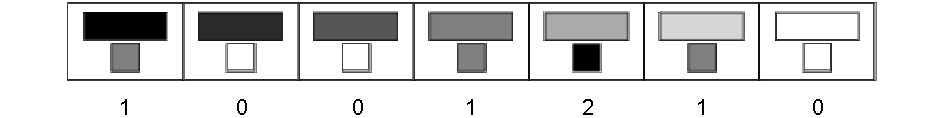
\includegraphics[width=0.7\textwidth]{fig_totalistcRule777.pdf}
	  \caption{Tabela de transição do AC totalístico 777. As transições dependem da média dos estados das células da vizinhança. Cada média possível é representada por tons de cinza entre o branco (estado 0) e o preto (estado 2).}
	  \label{fig:totalistcRule}
	\end{figure}

Já os ACs semi-totalísticos (\textit{outer-totalistic CA}) são generalizações de ACs totalísticos \cite{weisstein2015outerTotalistic}. Um AC é considerado semi-totalístico caso suas transições sejam definidas pela soma (ou média) das células da vizinhança sem levar em consideração a célula central.

\subsection{Confinamento}
Os autômatos celulares confinados (do inglês, \textit{captive}), são uma classe de ACs que se baseiam em uma caracterização de suas funções locais que não adotem estados definidos em qualquer estrutura externa à vizinhança \cite{theyssier2004captive}. 

\citeonline{theyssier2004captive} formalmente define que, dada a função local $f$ de um AC para a vizinhança $(\alpha_0, \dots, \alpha_{2r})$, sendo o $r$ o raio, um AC é considerado confinado se respeitar a condição descrita na Eq. \eqref{eq:captiveAC}.

\begin{equation}
f((\alpha_0, \dots, \alpha_{2r})) = \beta, \beta \in \{\alpha_0, \dots, \alpha_{2r}\}
\label{eq:captiveAC}
\end{equation}

Naturalmente, qualquer AC binário que tenha as funções locais $f((0_0, 0_1,\dots, 0_{2r})) = 0$ e $f((1_0, 1_,1\dots, 1_{2r})) = 1$ é um AC confinado.
